\setstretch{1}
\setlength{\parskip}{\baselineskip}

% ============================================================
%  Chapter 3 – System Architecture
% ============================================================

\section{Introduction}
\seclbl{arch-intro}
This chapter presents the architecture of the simulation system and the organization of its main functional components. The architecture is organized as a sequence of processing stages, each responsible for a specific task within the simulation flow. Such an organization improves ease of development while allowing individual components to be modified or extended with minimal impact on the rest of the system.

% ============================================================
\section{High-Level System Architecture}
\seclbl{arch-toplevel}
% ============================================================


As shown in Figure 3.2, the simulation process begins with a netlist file provided by the user. The netlist is first processed by the Netlist Parser, which reads the circuit description and extracts the required information, such as circuit elements, nodes, and simulation commands.

The extracted data is then passed to the Mathematical Modeling stage, where the circuit is converted into a mathematical form that can be analyzed by the simulator. This mathematical model is forwarded to the Simulation Engine, which performs the required calculations and generates the simulation results.

Next, the results are sent to the Post-Processing stage, where they are organized and prepared for display. Finally, the generated outputs are presented to the user.

The simulator can be used through different platforms, including a web application, a desktop application, and Linux-based systems. Regardless of the platform, the same simulation flow is followed.

\begin{figure}[H]
    \centering
    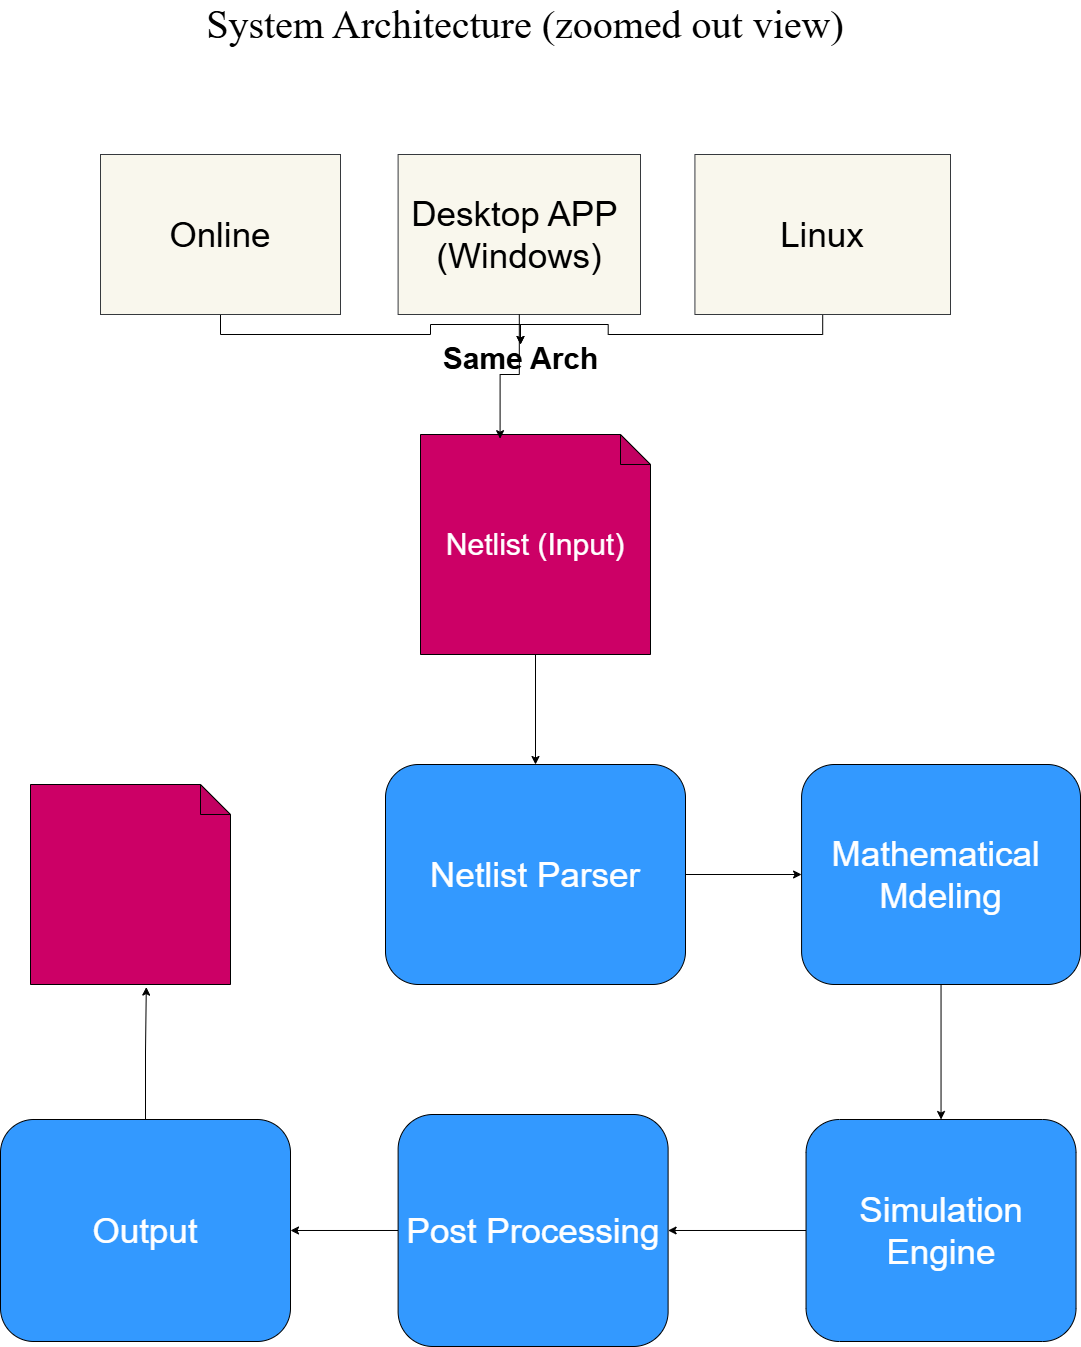
\includegraphics[width=0.8\textwidth]{Figures/Ch3/High_level_arch.drawio}
      \renewcommand{\thefigure}{3.2}
    \addtocounter{figure}{-1}
    \caption{Top-level System Architecture.}
    \label{fig:arch-toplevel}
\end{figure}


   

% ============================================================
\section{Detailed System Architecture}
\seclbl{arch-Detailed}

\begin{figure}[H]
    \centering
    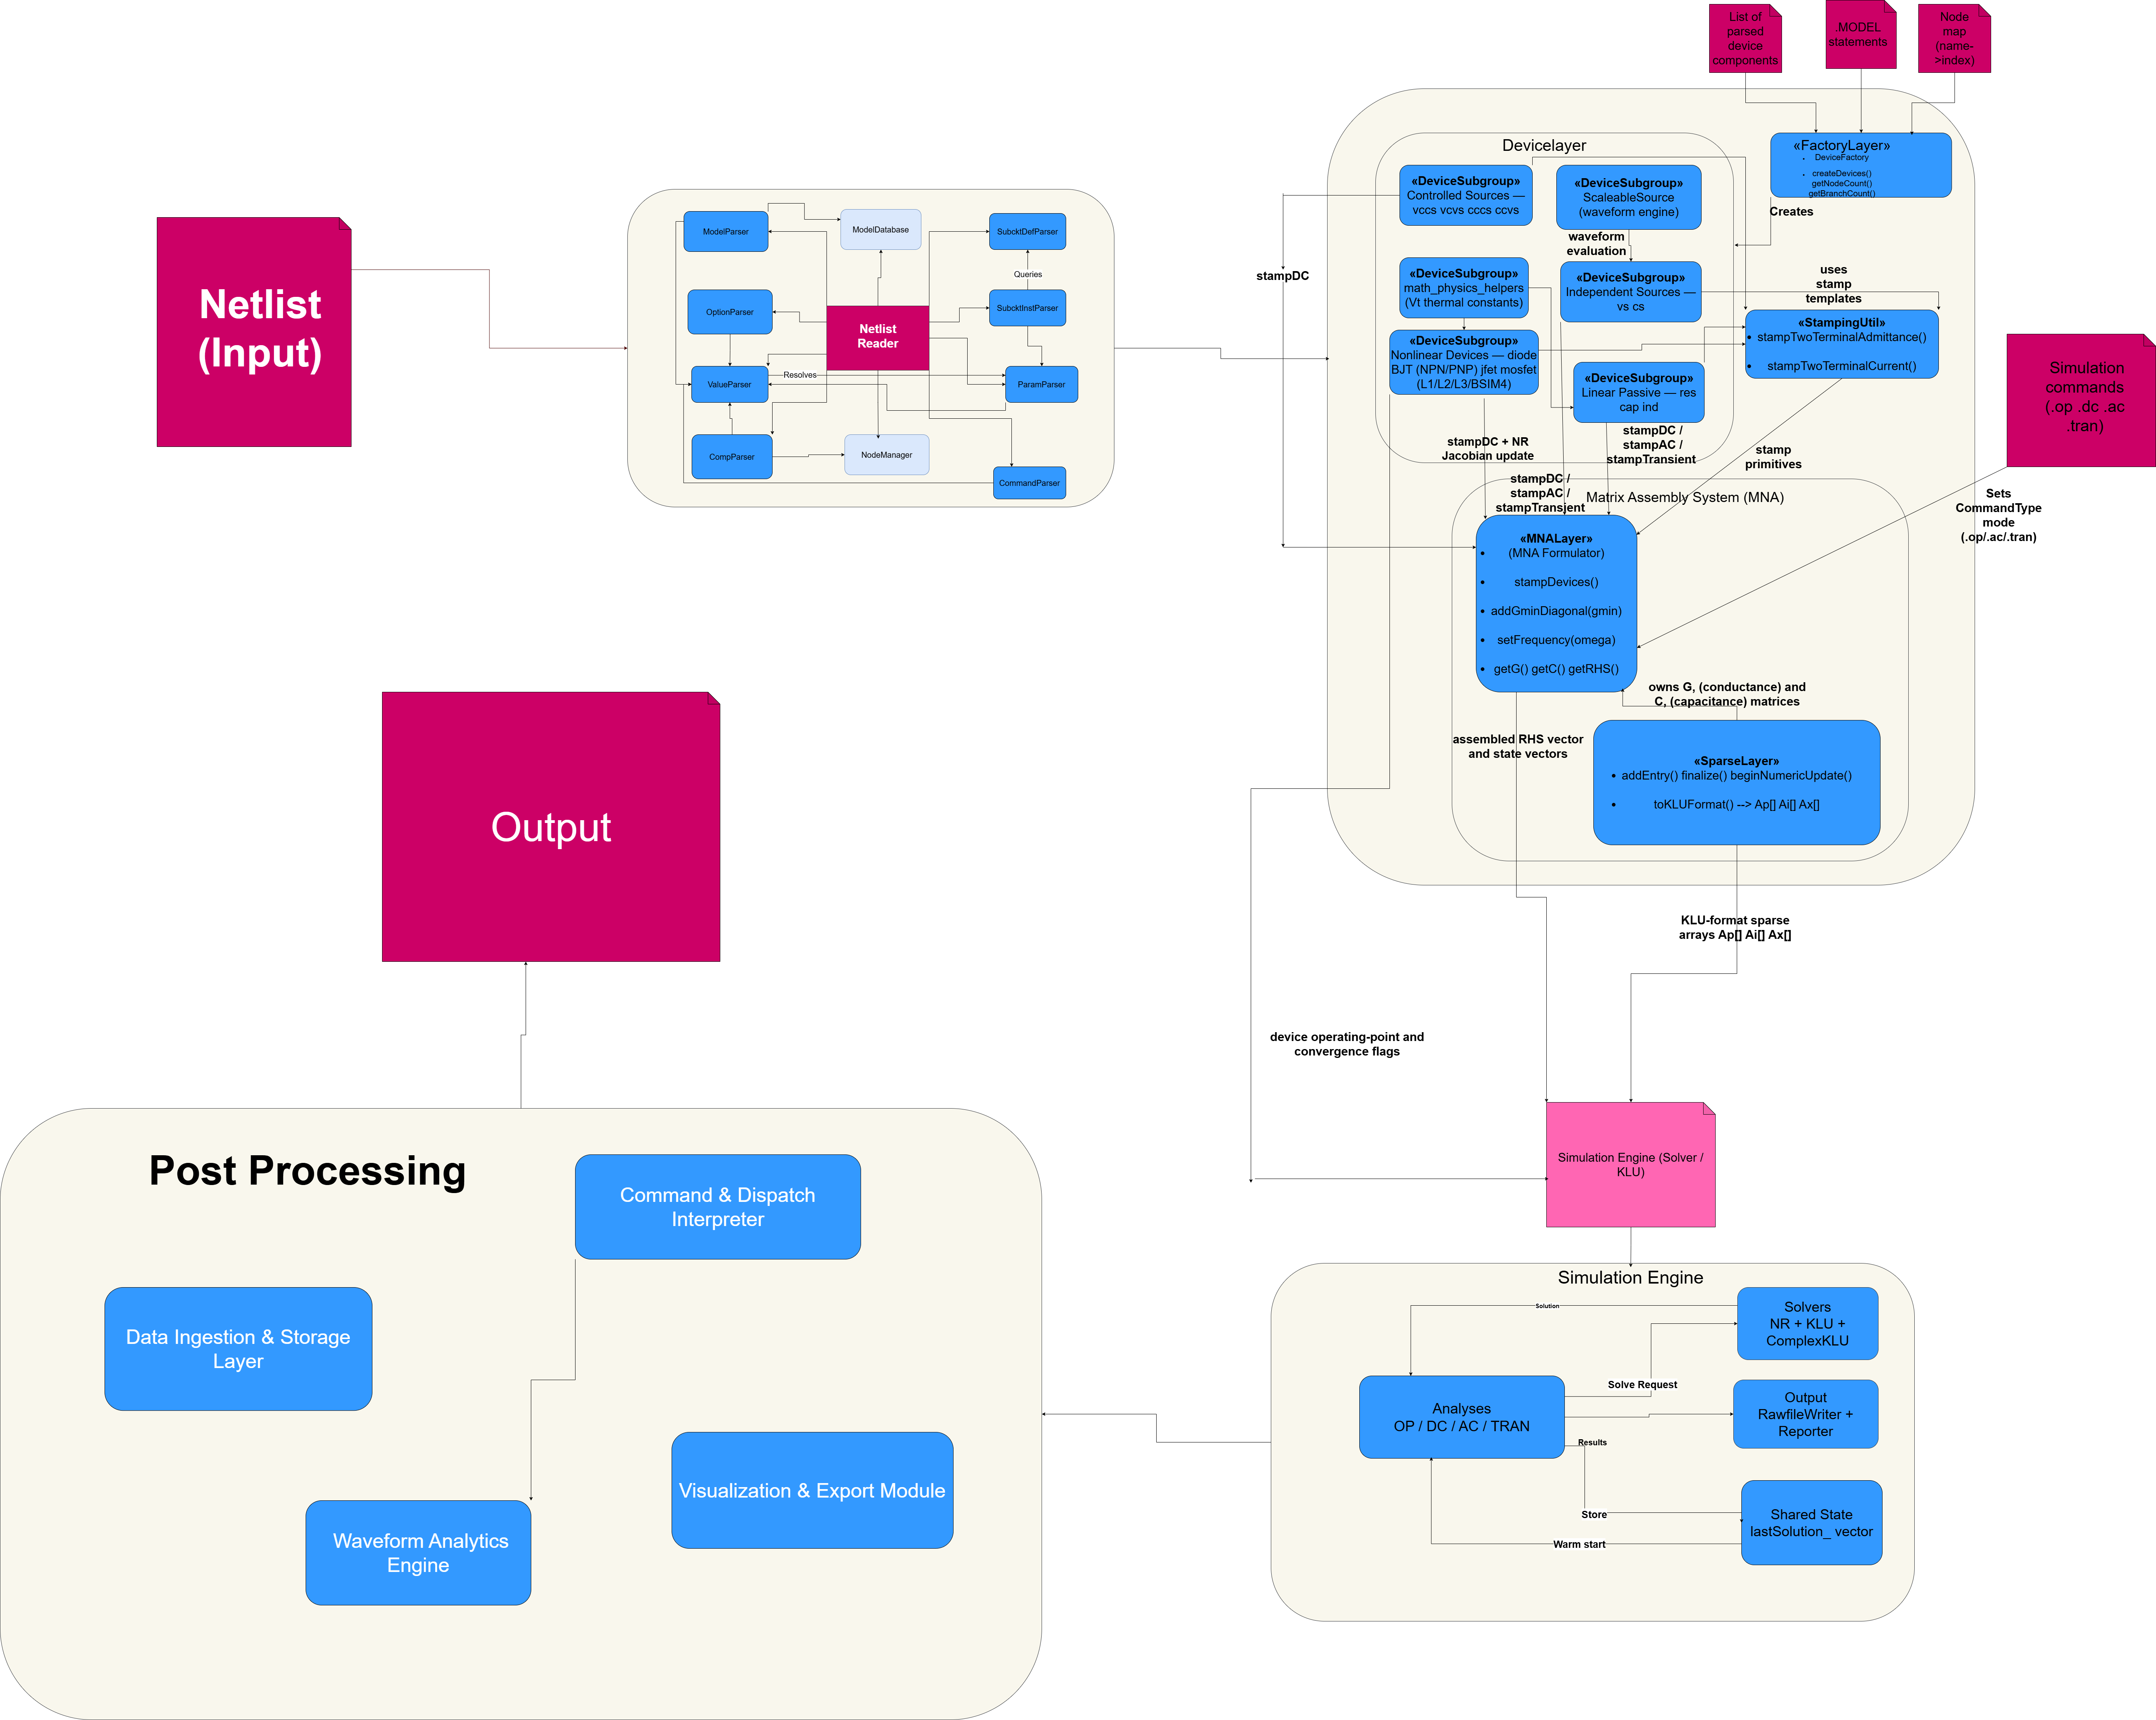
\includegraphics[width=0.8\textwidth]{Figures/Ch3/Detailed.ARCH.drawio}
    \renewcommand{\thefigure}{3.3}
    \addtocounter{figure}{-1}
    \caption{Detailed System Architecture.}
    \label{fig:arch-detailed}
\end{figure}

% ============================================================

\subsection{Netlist Parser Subsystem}
\seclbl{arch-Detailed-Netlist}
% ============================================================
\subsubsection{Overview}
\seclbl{arch-netlist-overview}
% ============================================================
The Netlist Parser is the first stage of the simulation framework and is responsible for converting the textual SPICE netlist into structured data that can be processed by the simulation engine. It reads the input netlist line by line, identifies the different statement types, and dispatches them to specialized parser modules according to their functionality. These modules handle component definitions, simulation options, parameter values, device models, subcircuit definitions and instantiations, and simulation control commands.
The output of this stage is a complete internal representation of the circuit, including all devices, nodes, simulation options, models, and control commands, which is then passed to the Simulation Engine for numerical analysis.
% ============================================================
\subsubsection{NetlistReader}
\seclbl{arch-netlist-reader}
% ============================================================
The NetlistReader is the main controller of the Netlist Parser. It reads the SPICE netlist line by line, identifies the type of each statement, and sends it to the appropriate parser module for processing. It also coordinates the communication between the parser modules, ensuring that all circuit information is correctly organized before being passed to the simulation engine.

% ============================================================
\subsubsection{ModelParser \& ModelDatabase}
\seclbl{arch-netlist-model}
% ============================================================
The ModelParser is responsible for parsing all .MODEL statements in the SPICE netlist. These statements define the electrical characteristics of semiconductor devices, such as diodes, BJTs, and MOSFETs. After extracting the model name, device type, and associated parameters, the parser stores the information in the ModelDatabase. The ModelDatabase acts as a centralized repository that allows other parser modules, particularly the CompParser, to retrieve the required model whenever a device references it.

% ============================================================
\subsubsection{OptionParser}
\seclbl{arch-netlist-option}
% ============================================================
The OptionParser is responsible for parsing the .OPTIONS statements in the SPICE netlist. These statements specify simulation settings that control the behavior and accuracy of the simulator, such as numerical tolerances and solver options. The parser extracts each option and its corresponding value, converts numerical values using the ValueParser when necessary, and stores the parsed settings so they can be used during the simulation process.

% ============================================================
\subsubsection{ValueParser}
\seclbl{arch-netlist-value}
% ============================================================
The ValueParser is responsible for converting the values written in the SPICE netlist into numerical values that can be used by the simulator. It recognizes engineering prefixes such as k, m, u, n, and p, ensuring that component values and simulation parameters are interpreted correctly. It also helps resolve parameter values and expressions when needed. It is used by several parser modules, including the CompParser, OptionParser, and ParamParser.

% ============================================================
\subsubsection{CompParser \& NodeManager}
\seclbl{arch-netlist-comp}
% ============================================================
The CompParser is responsible for parsing the circuit components defined in the SPICE netlist, such as resistors, capacitors, inductors, voltage sources, current sources, diodes, MOSFETs, and BJTs. For each component, it extracts the component name, connected nodes, and associated parameters before creating the corresponding internal circuit object. During this process, the NodeManager assigns a unique numerical index to each node name, ensuring that all circuit components use a consistent node numbering scheme. Together, these modules transform the textual circuit description into an internal circuit representation that can be processed by the simulation engine.

% ============================================================
\subsubsection{SubcktDefParser \& SubcktInstParser}
\seclbl{arch-netlist-subckt}
% ============================================================
The SubcktDefParser and SubcktInstParser work together to support hierarchical circuit design in the SPICE netlist. The SubcktDefParser processes .SUBCKT definitions, extracting the subcircuit name, external terminals, and internal components, and stores the complete definition for later use. The SubcktInstParser processes subcircuit instances, which are identified by lines beginning with X, and creates circuit instances based on the previously stored definitions. During this process, the external nodes of the instance are mapped to the corresponding terminals of the subcircuit, allowing the same circuit block to be reused multiple times within a design.

% ============================================================
\subsubsection{ParamParser}
\seclbl{arch-netlist-param}
% ============================================================
The ParamParser is responsible for parsing .PARAM statements in the SPICE netlist. These statements define user parameters that can be referenced by circuit components and other expressions. The parser extracts the parameter name and its corresponding value, converts the value when necessary using the ValueParser, and stores the parameter for later use. During parsing, any reference to a parameter is replaced with its corresponding numerical value, ensuring that all circuit components receive valid values before simulation.

% ============================================================
\subsubsection{CommandParser}
\seclbl{arch-netlist-command}
% ============================================================
The CommandParser is responsible for processing simulation control commands in the SPICE netlist. These commands specify the type of analysis to be performed, such as DC, AC, Transient, or Operating Point analysis. The parser extracts the command type and its associated parameters, validates the input, and stores the simulation configuration so that the appropriate analysis can be executed by the simulation engine.






\begin{figure}[H]
    \centering
    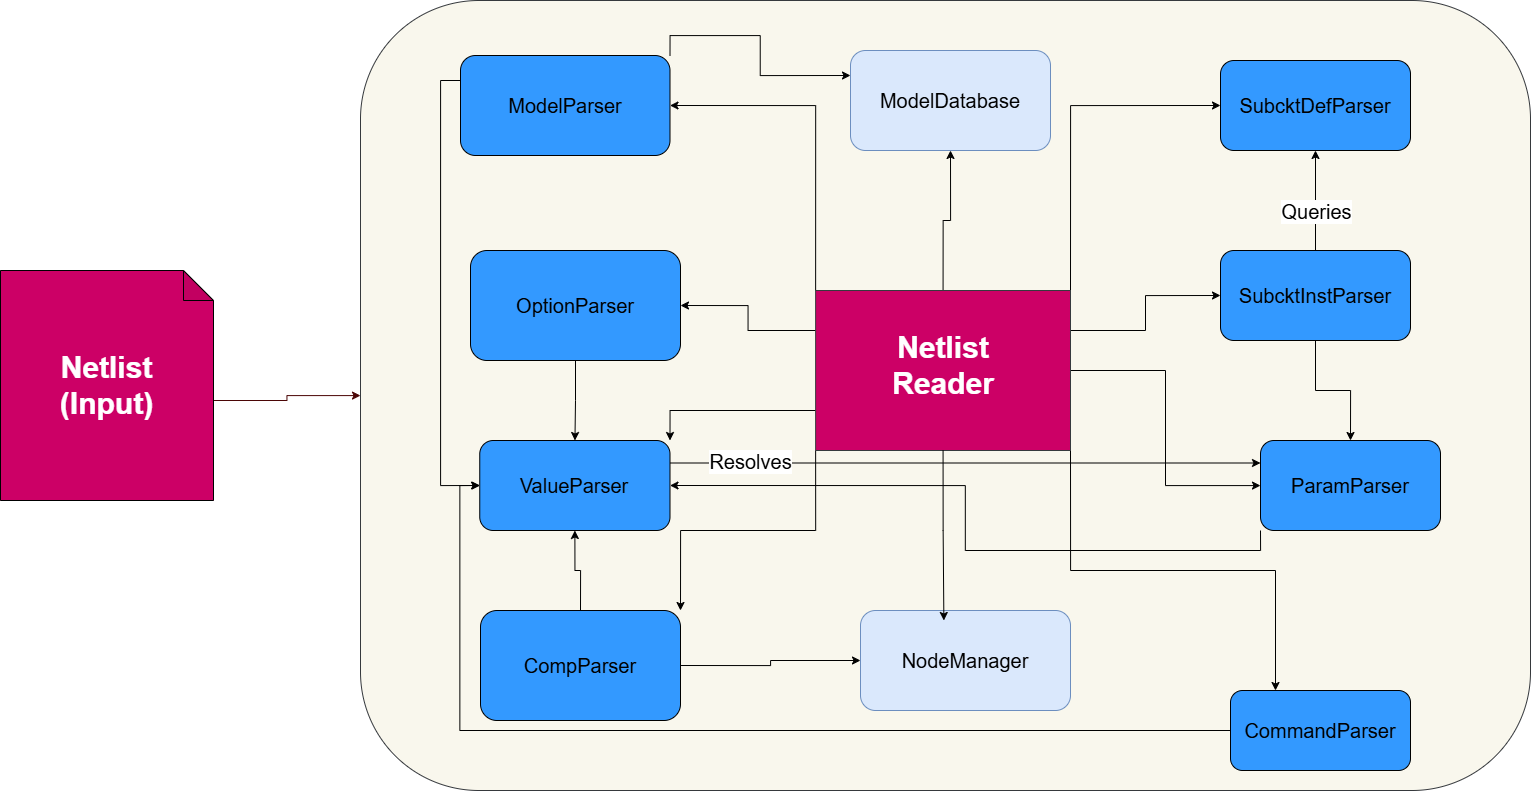
\includegraphics[width=0.8\textwidth]{Figures/Ch3/netlist_parser.drawio}
    \renewcommand{\thefigure}{3.3.1}
    \addtocounter{figure}{-1}
    \caption{ Netlist Parser stage.}
    \label{fig:arch-netlist}
\end{figure}
% ============================================================
\subsection{Mathematical Modeling Subsystem}
\seclbl{arch-Detailed-Modeling}
% ============================================================

% ============================================================
\subsubsection{Overview}
\seclbl{arch-modeling-overview}
% ============================================================
The Mathematical Modeling stage transforms the parsed circuit description into a mathematical representation that can be solved by the Simulation Engine. It receives the parsed circuit components, model definitions, node mapping information, and simulation commands from the Netlist Parser. Based on these inputs, the stage creates the appropriate device models, computes the mathematical contribution of each device, and assembles all contributions into a global Modified Nodal Analysis (MNA) matrix. The completed matrix representation is then passed to the Simulation Engine for numerical solution.
% ============================================================
\subsubsection{DeviceFactory}
\seclbl{arch-modeling-devicefactory}
% ============================================================
The DeviceFactory serves as the entry point of the Mathematical Modeling stage. As shown in Figure 3.3.2, it receives three main inputs: the parsed device components, the model definitions stored in the ModelDatabase, and the node map generated during the netlist parsing stage. The parsed components provide the type, connectivity, and parameters of each circuit element, while the model definitions supply the electrical parameters required for nonlinear devices such as diodes, BJTs, and MOSFETs. The node map provides the numerical indices assigned to circuit nodes, which are required during matrix assembly.

Using these inputs, the DeviceFactory identifies the type of each circuit element and creates the corresponding mathematical device object.This process represents the electrical behavior of each component into a dedicated device model that can later contribute its equations to the circuit formulation.

After creating the device objects, the DeviceFactory forwards them to the Device Layer. Each object is routed to its corresponding device category, including Independent Sources, Controlled Sources, Linear Passive Devices, or Nonlinear Devices, depending on its electrical type. 

In addition to creating device objects, the DeviceFactory maintains the total number of circuit nodes and branch variables through the getNodeCount() and getBranchCount() interfaces. This information is later used by the MNA Formulator to allocate the global circuit matrices with the appropriate dimensions before the device equations are assembled
% ============================================================
\subsubsection{Device Layer (Device Models)}
\seclbl{arch-modeling-devicelayer}
% ============================================================

% ============================================================
\paragraph{Overview}
\seclbl{arch-modeling-devicelayer-overview}
% ============================================================
The Device Layer contains the mathematical implementations of all circuit elements supported by the simulator. As shown in Figure 3.3.2, the device objects created by the DeviceFactory are forwarded to the appropriate device category according to their electrical characteristics.
Each device computes the mathematical equations that describe its electrical behavior. These equations are then passed to the Stamping Utilities, which insert the corresponding values into the appropriate positions of the Modified Nodal Analysis (MNA) matrix. Separating device modeling from matrix assembly keeps each device focused on its own electrical behavior and makes the simulator easier to maintain and extend.
% ============================================================
\paragraph{Linear Passive Devices}
\seclbl{arch-modeling-devicelayer-linear}
% ============================================================
The Linear Passive Devices module models passive circuit elements such as resistors, capacitors, and inductors. After receiving the corresponding device objects from the DeviceFactory, each device computes the mathematical equations describing its electrical behavior according to the selected analysis type. Instead of directly modifying the global circuit matrix, these equations are forwarded to the Stamping Utilities, which insert the corresponding matrix contributions into the Modified Nodal Analysis formulation.
% ============================================================
\paragraph{Independent Sources}
\seclbl{arch-modeling-devicelayer-indepsource}
% ============================================================
The Independent Sources module models circuit elements whose output is specified independently of any other circuit variable, such as independent voltage and current sources. After receiving the corresponding device objects from the DeviceFactory, each source computes its mathematical contribution according to its specified value. These contributions are then forwarded to the Stamping Utilities, where they are incorporated into the Modified Nodal Analysis (MNA) matrix.
% ============================================================
\paragraph{Controlled Sources}
\seclbl{arch-modeling-devicelayer-ctrlsource}
% ============================================================
The Controlled Sources module models dependent sources whose output is controlled by another voltage or current in the circuit. This includes voltage-controlled and current-controlled voltage and current sources. Based on the controlling signal, each device computes its mathematical contribution and forwards it to the Stamping Utilities, which insert the corresponding equations into the MNA matrix.
% ============================================================
\paragraph{Nonlinear Devices}
\seclbl{arch-modeling-devicelayer-nonlinear}
% ============================================================
The Nonlinear Devices module models semiconductor devices such as diodes, BJTs, JFETs, and MOSFETs. These devices use nonlinear mathematical models to describe their electrical behavior. Since their equations depend on the operating point of the circuit, their mathematical contributions are recalculated iteratively during the simulation until a converged solution is obtained. At each iteration, the updated contributions are passed to the Stamping Utilities, which incorporate them into the MNA matrix.
% ============================================================
\paragraph{ScalableSource}
\seclbl{arch-modeling-devicelayer-scalable}
% ============================================================
The ScalableSource module provides shared functionality for source devices that require common operations, such as scaling or evaluating parameterized source values. After the required calculations are completed, the source devices continue generating their mathematical contributions, which are then forwarded to the Stamping Utilities for insertion into the MNA matrix.
% ============================================================
\paragraph{math\_physics\_helpers}
\seclbl{arch-modeling-devicelayer-helpers}
% ============================================================
The math\_physics\_helpers module provides shared mathematical and physical utility functions used by multiple device models during equation evaluation. It includes common calculations, physical constants, and helper routines that are required by several device implementations, particularly nonlinear semiconductor devices. By centralizing these functions.
% ============================================================
\subsubsection{Stamping Utilities}
\seclbl{arch-modeling-stamping}
% ============================================================
The Stamping Utilities module provides a common mechanism for inserting the mathematical contributions of all device models into the global Modified Nodal Analysis (MNA) matrix. As illustrated in Figure 3.3.2, it receives the computed equations from Devices. the Stamping Utilities determine the appropriate matrix locations based on the device connections and update the corresponding matrix entries. Once the contributions of all devices have been inserted, the completed matrix is forwarded to the MNA Formulator for constructing the final system of circuit equations.
% ============================================================
\subsubsection{Matrix Assembly System (MNA Formulation)}
\seclbl{arch-modeling-matrixassembly}
% ============================================================
\paragraph{Overview}
\seclbl{arch-modeling-matrixassembly-overview}
% ============================================================
The MNA Assembly stage is responsible for constructing the complete mathematical representation of the circuit after the device contributions have been generated. it receives the stamped contributions from the Stamping Utilities and organizes them through two complementary layers. The MNA Layer and the Sparse Layer.
% ============================================================
\paragraph{MNA layer}
\seclbl{arch-modeling-matrixassembly-mna}
% ============================================================
The MNA Layer is responsible for assembling the complete Modified Nodal Analysis representation of the circuit. It receives the stamped device contributions from the Stamping Utilities and combines them into the global circuit equations. This layer constructs the conductance matrix (G), the dynamic matrix (C), and the excitation vector (RHS), while also managing different simulation modes such as operating point, DC, AC, and transient analyses. During transient simulation, it updates the device states before assembling the new matrix equations. Once all device contributions have been assembled, the resulting matrices are forwarded to the Sparse Layer for efficient storage and numerical processing.
% ============================================================
\paragraph{Sparse layer}
\seclbl{arch-modeling-matrixassembly-sparse}
% ============================================================
The Sparse Layer, converts the assembled MNA matrices into a compressed sparse representation suitable for efficient numerical computation. It receives the conductance and dynamic matrices from the MNA Layer and stores only their non-zero entries using a compressed sparse column (CSC) format. During this process, duplicate entries are merged, zero-valued elements are removed, and the sparse matrix structure is finalized. The resulting sparse matrices significantly reduce memory usage and computational complexity, making them suitable for direct solution by the KLU Sparse Matrix solver.

\begin{figure}[H]
    \centering
    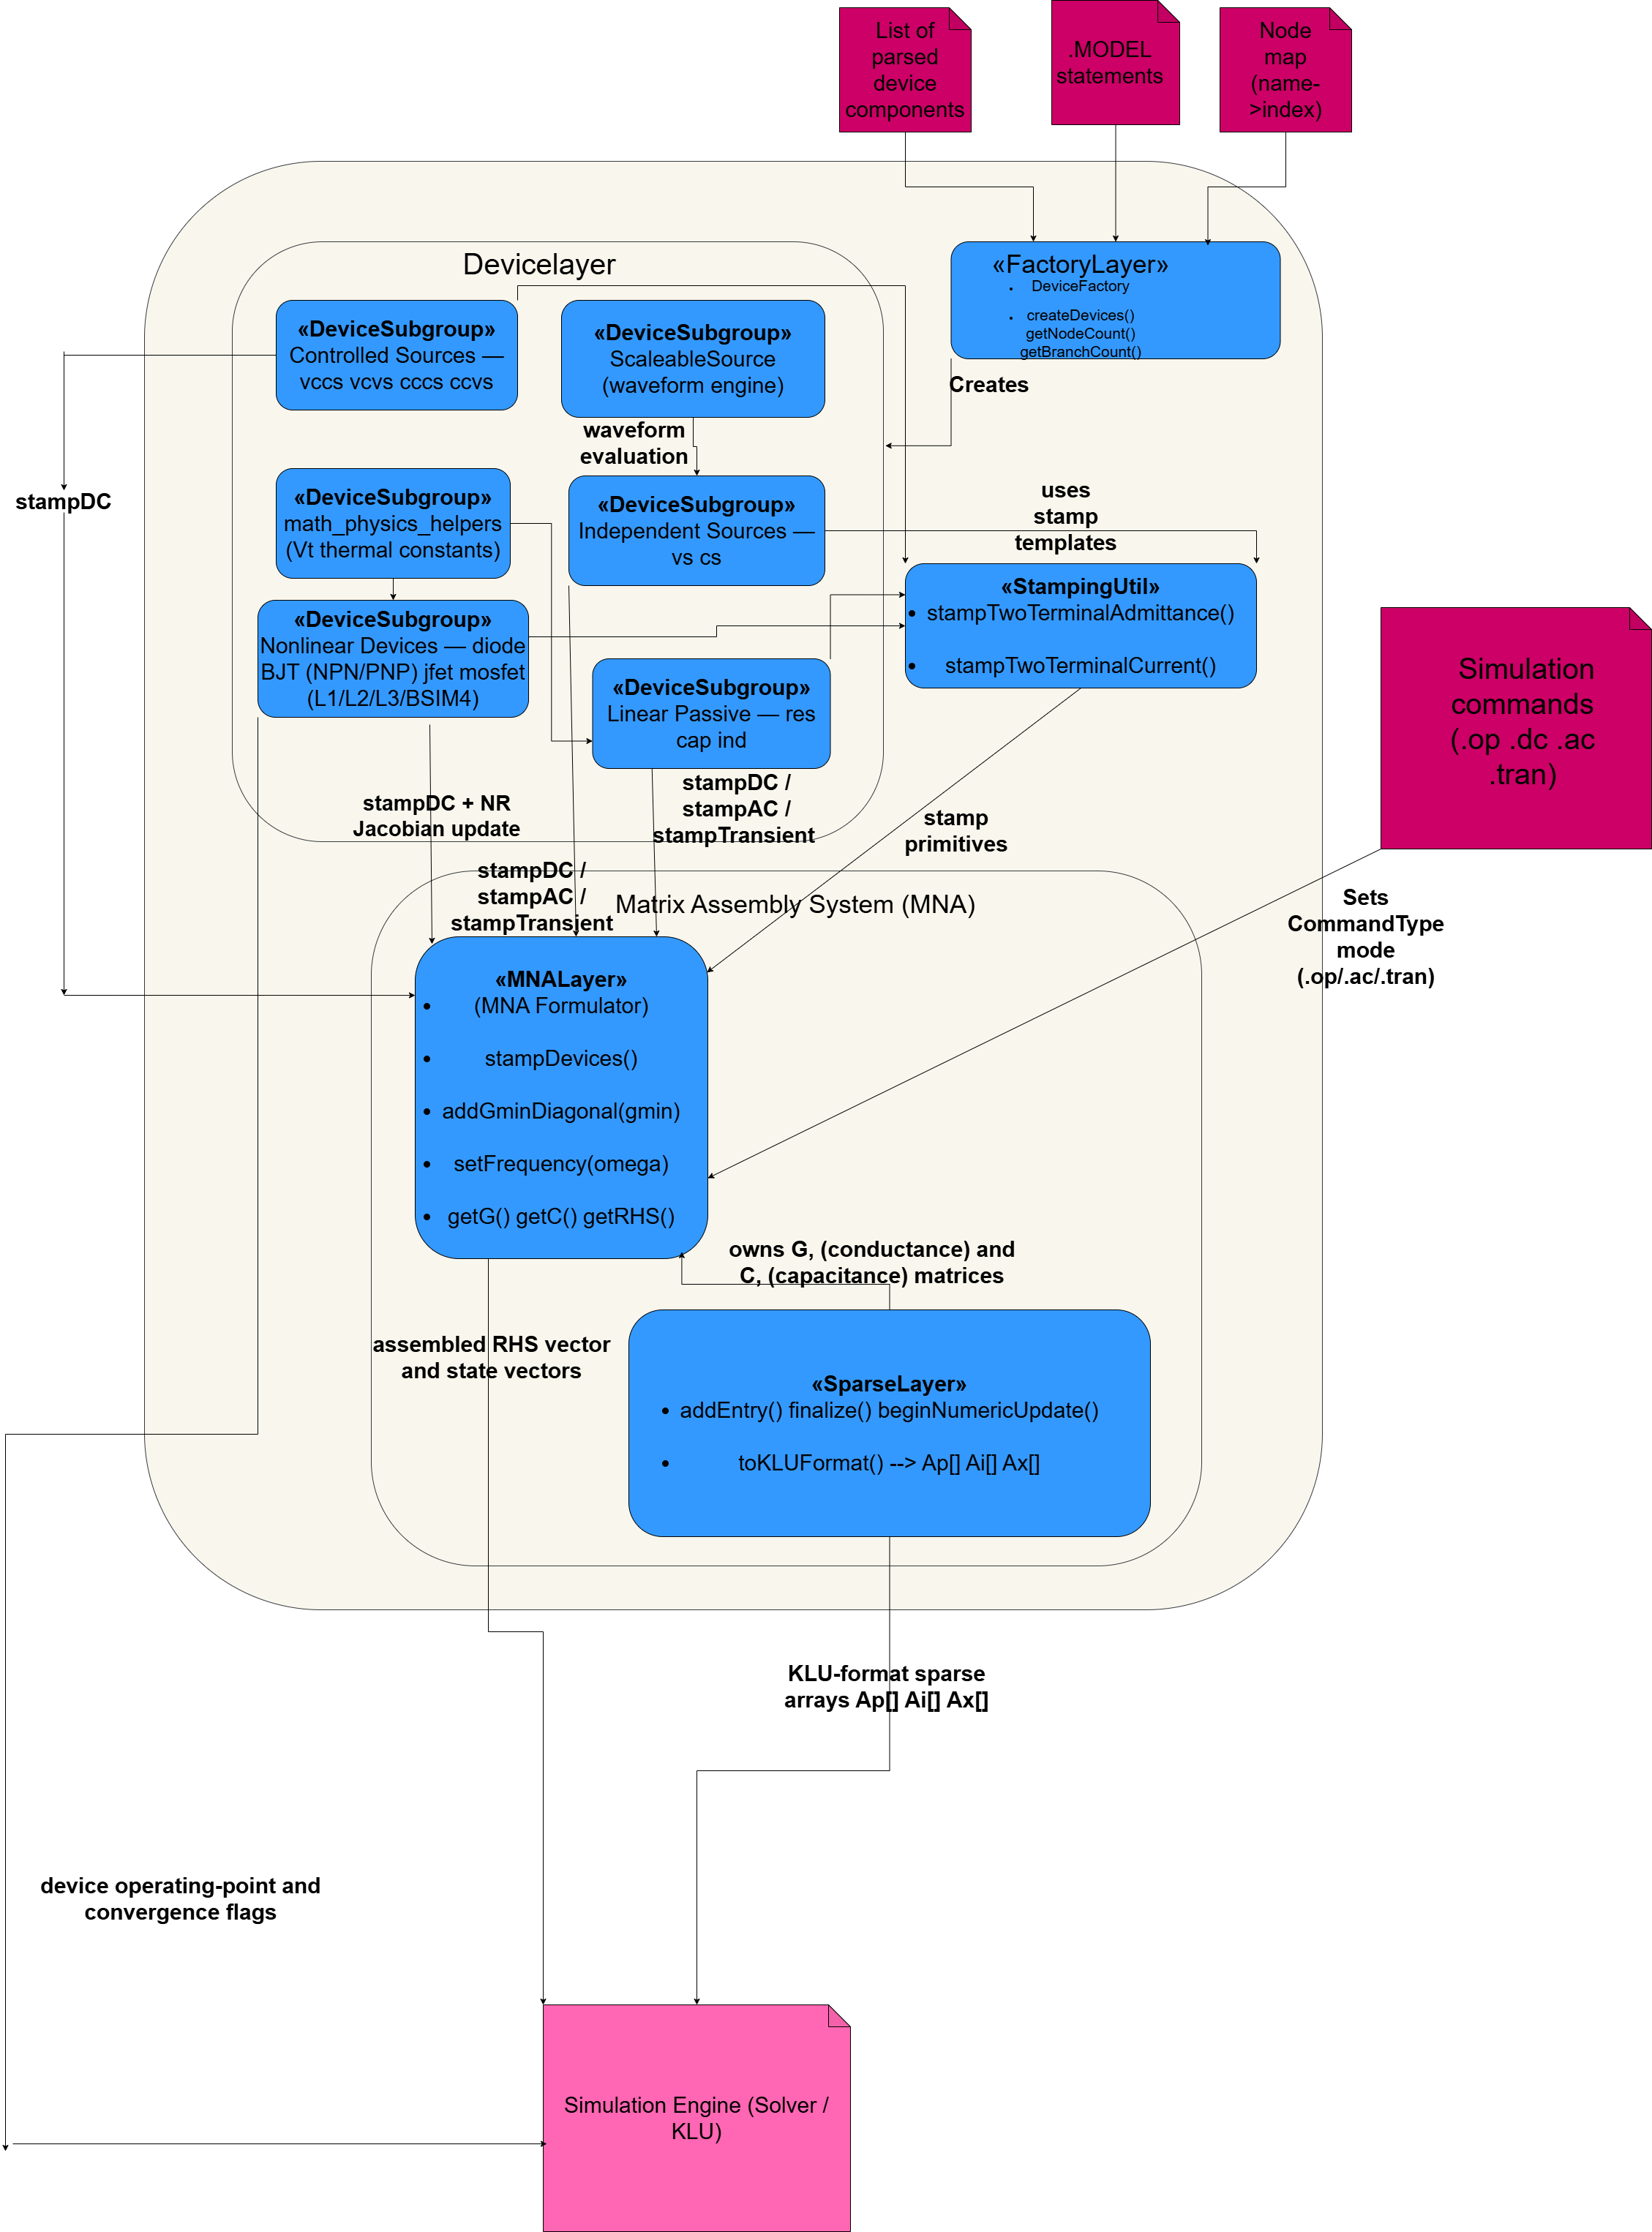
\includegraphics[width=\textwidth]{Figures/Ch3/MM.drawio.png}
    \renewcommand{\thefigure}{3.3.2}
    \addtocounter{figure}{-1}
    \caption{ Mathematical Modeling stage.}
    \label{fig:arch-mathmodel}
\end{figure}


% ============================================================
\subsection{Simulation Engine Architecture}
\seclbl{arch-engine}
% ============================================================

% ============================================================
\subsubsection{Overview}
\seclbl{arch-engine-overview}
% ============================================================
The Simulation Engine performs the numerical analysis of the mathematical circuit model generated during the Mathematical Modeling stage. It supports four types of circuit analyses: Operating Point (OP), DC Sweep, AC, and Transient (TRAN) analysis. The Analyses module acts as the central controller, selecting the requested analysis according to the simulation command. Depending on the analysis type, it communicates with the appropriate numerical solver to obtain the circuit solution, stores the computed solution for reuse in subsequent analyses, and forwards the final simulation results to the output module for reporting and waveform generation.
 % ============================================================
\subsubsection{Analysis}
\seclbl{arch-engine-analysis}
% ============================================================
The Analyses module serves as the main controller of the Simulation Engine. It receives the mathematical circuit representation from the Mathematical Modeling stage together with the requested simulation command, and determines which analysis should be executed. Once the appropriate analysis is selected, the module sends a solve request to the corresponding solver and waits for the computed solution. 
% ============================================================
\subsubsection{Solvers}
\seclbl{arch-engine-solvers}
% ============================================================
% ============================================================
\paragraph{NR (Newton-Raphson)}
\seclbl{arch-engine-solvers-nr}
% ============================================================
The Newton–Raphson (NR) solver is responsible for solving nonlinear circuit equations involving devices such as diodes, BJTs, and MOSFETs. Upon receiving a solve request from the Analyses module, it repeatedly linearizes the nonlinear device equations around the current operating point and computes an updated solution until the convergence criteria are satisfied. During each iteration, the NR solver invokes the KLU solver to solve the resulting linearized sparse system of equations. Once convergence is achieved, the final solution is returned to the Analyses module.
% ============================================================
\paragraph{KLU Solver}
\seclbl{arch-engine-solvers-klu}
% ============================================================
The KLU solver performs the numerical solution of sparse real-valued linear systems generated during circuit simulation. It receives the sparse matrices assembled by the Mathematical Modeling stage, either directly for linear analyses or from the Newton–Raphson solver during each nonlinear iteration. The KLU solver efficiently factorizes the sparse matrix and computes the unknown node voltages and branch currents. The computed solution is then returned to the requesting analysis or to the Newton–Raphson solver for further iterations.
% ============================================================
\paragraph{ComplexKLU Solver}
\seclbl{arch-engine-solvers-complexklu}
% ============================================================
The ComplexKLU solver extends the functionality of the KLU solver to support complex-valued sparse matrices generated during AC analysis. Since AC analysis represents circuit quantities in the frequency domain using complex numbers, the assembled MNA matrices contain both real and imaginary components. The ComplexKLU solver efficiently solves these complex linear systems and returns the frequency-domain solution to the Analyses module.
% ============================================================
\subsubsection{Shared State}
\seclbl{arch-engine-sharedstate}
% ============================================================
The Shared State module stores the current simulation solution and other shared data that may be required by multiple analyses. After each successful solution, the Analyses module stores the computed node voltages and branch currents in the Shared State. During later simulation steps, such as DC sweep  or transient Analysis, the stored solution is retrieved and used as the initial guess for the next numerical solution. This warm-start mechanism reduces the number of solver iterations, improves convergence, and increases the overall simulation efficiency by avoiding repeated initialization from scratch.







\begin{figure}[H]
    \centering
    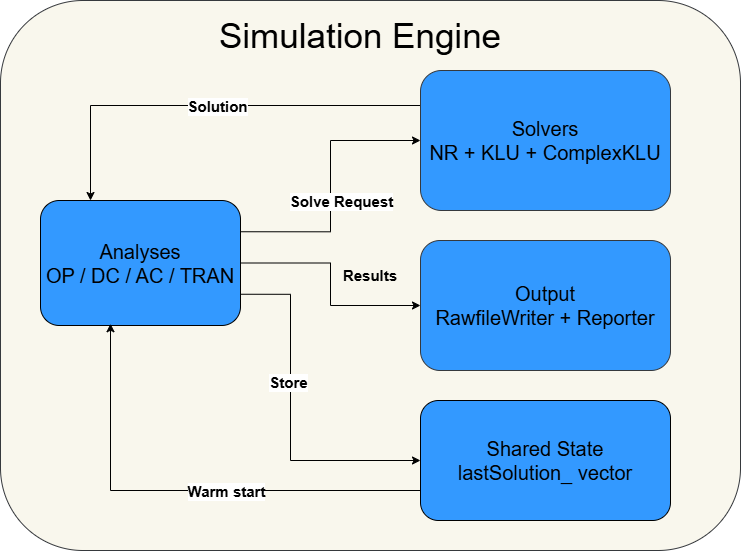
\includegraphics[width=0.8\textwidth]{Figures/Ch3/SIM.drawio}
    \renewcommand{\thefigure}{3.3.3}
    \addtocounter{figure}{-1}
    \caption{ Simulation Engine stage.}
    \label{fig:arch-engine}
\end{figure}
% ============================================================
\subsection{Post-Processing Architecture}
\seclbl{arch-postproc}
% ============================================================
% ============================================================
\subsubsection{Overview}
\seclbl{arch-postproc-overview}
% ============================================================
The Post-Processing Stage is responsible for transforming raw simulation output into meaningful numerical and graphical results that enable users to analyze circuit behavior efficiently.
The Post-Processing Stage is organized into four main sections: the Data Ingestion \& Storage Layer, which imports and stores simulation results; the Command \& Dispatch Interpreter, which parses and routes user commands; the Waveform Analytics Engine, which performs waveform measurements and mathematical calculations; and the Visualization \& Export Module, which presents the processed results through plots, printed waveform data, or exported files.
% ============================================================
\subsubsection{Data Ingestion and Storage Layer}
\seclbl{arch-postproc-ingestion}
% ============================================================
The Data Ingestion and Storage Layer serves as the entry point of the post-processing stage. Its primary responsibility is to import the simulation results generated by the simulation engine and organize them into an internal database for subsequent analysis and visualization. This process begins with the RawfileReader, which reads the generated SPICE-compatible RAW file. The reader first parses the file header to extract simulation metadata, including the analysis type, number of variables, number of simulation points, and other descriptive information. It then reads the list of recorded signals, such as node voltages, branch currents, and the sweep variable (e.g., time for transient analysis or frequency for AC analysis), before loading the corresponding binary waveform samples into memory. The parsed data is organized into a structured RawFile object, which represents a complete simulation result. This object is then transferred to the WaveformDB, which acts as a centralized waveform repository. WaveformDB stores all waveform data and metadata, and supports storing newly generated waveforms produced during mathematical processing. In addition, this layer provides user commands such as load, source, info, list, and db, allowing users to load simulation results, execute netlists, inspect simulation metadata, list available signals, and manage the waveform database. By separating data loading from subsequent processing, this layer establishes a consistent and reusable data source for the remaining post-processing modules

% ============================================================
\subsubsection{Command \& Dispatch Interpreter}
\seclbl{arch-postproc-interpreter}
% ============================================================
The Command \& Dispatch Interpreter serves as the central control unit of the post-processing stage, acting as the interface between the user and the waveform processing modules. It receives commands entered through the command-line interface, tokenizes and validates the input, identifies the requested operation, and dispatches the command to the appropriate module for execution. Depending on the command type, requests related to waveform management are directed to the WaveformDB, numerical measurements are handled by the Waveform Analytics Engine, while plotting and data export operations are forwarded to the Visualization \& Export Module. To support different user workflows, the interpreter operates in REPL (Read-Evaluate-Print Loop) mode for interactive command execution, Script mode for automated execution of command sequences from script files, and CLI (Command-Line Interface) mode for executing individual commands directly from the terminal. Furthermore, the interpreter enhances usability through comprehensive command validation, descriptive error reporting, and fuzzy string-matching based on the Levenshtein distance algorithm, enabling it to suggest the closest valid command or signal name when typographical errors occur. This modular command-dispatch mechanism simplifies user interaction while ensuring that each request is efficiently routed to the appropriate processing component.


% ============================================================
\subsubsection{Waveform Analytics Engine}
\seclbl{arch-postproc-analytics}
% ============================================================
The Waveform Analytics Engine is responsible for performing numerical analysis and mathematical processing on waveform data stored in the WaveformDB. Upon receiving analysis-related commands from the Command \& Dispatch Interpreter, the engine retrieves the requested signals and executes the appropriate processing operation. The engine consists of two complementary modules. The MeasEngine extracts numerical characteristics from waveforms, including maximum and minimum values, peak-to-peak voltage, average, RMS, rise and fall times, crossing points, period, frequency, propagation delay, and signal values at specified coordinates. These operations produce scalar measurement results that characterize circuit behavior. In contrast, the CalcEngine evaluates mathematical expressions involving one or more waveforms, supporting arithmetic operations as well as mathematical functions such as square root, logarithm, absolute value, and decibel conversion. Unlike measurement operations, calculation operations generate new derived waveforms, which are subsequently stored in the WaveformDB for further analysis, visualization, or export.


% ============================================================
\subsubsection{Visualization \& Export Module}
\seclbl{arch-postproc-visualization}
% ============================================================
The Visualization \& Export Module is the final stage of the post-processing pipeline. After waveform data has been imported, stored, and analyzed, this module is responsible for presenting the processed results to the user in a readable and useful format. It retrieves waveform data and analysis results from the WaveformDB, then either displays them numerically, generates graphical plots, or exports them to external files for further processing. Unlike the previous stages, which focus on data management and numerical computation, this module focuses on presenting the results. It therefore serves as the interface between the internal waveform processing system and the user, allowing simulation results to be interpreted visually or transferred to other analysis tools



\begin{figure}[H]
    \centering
    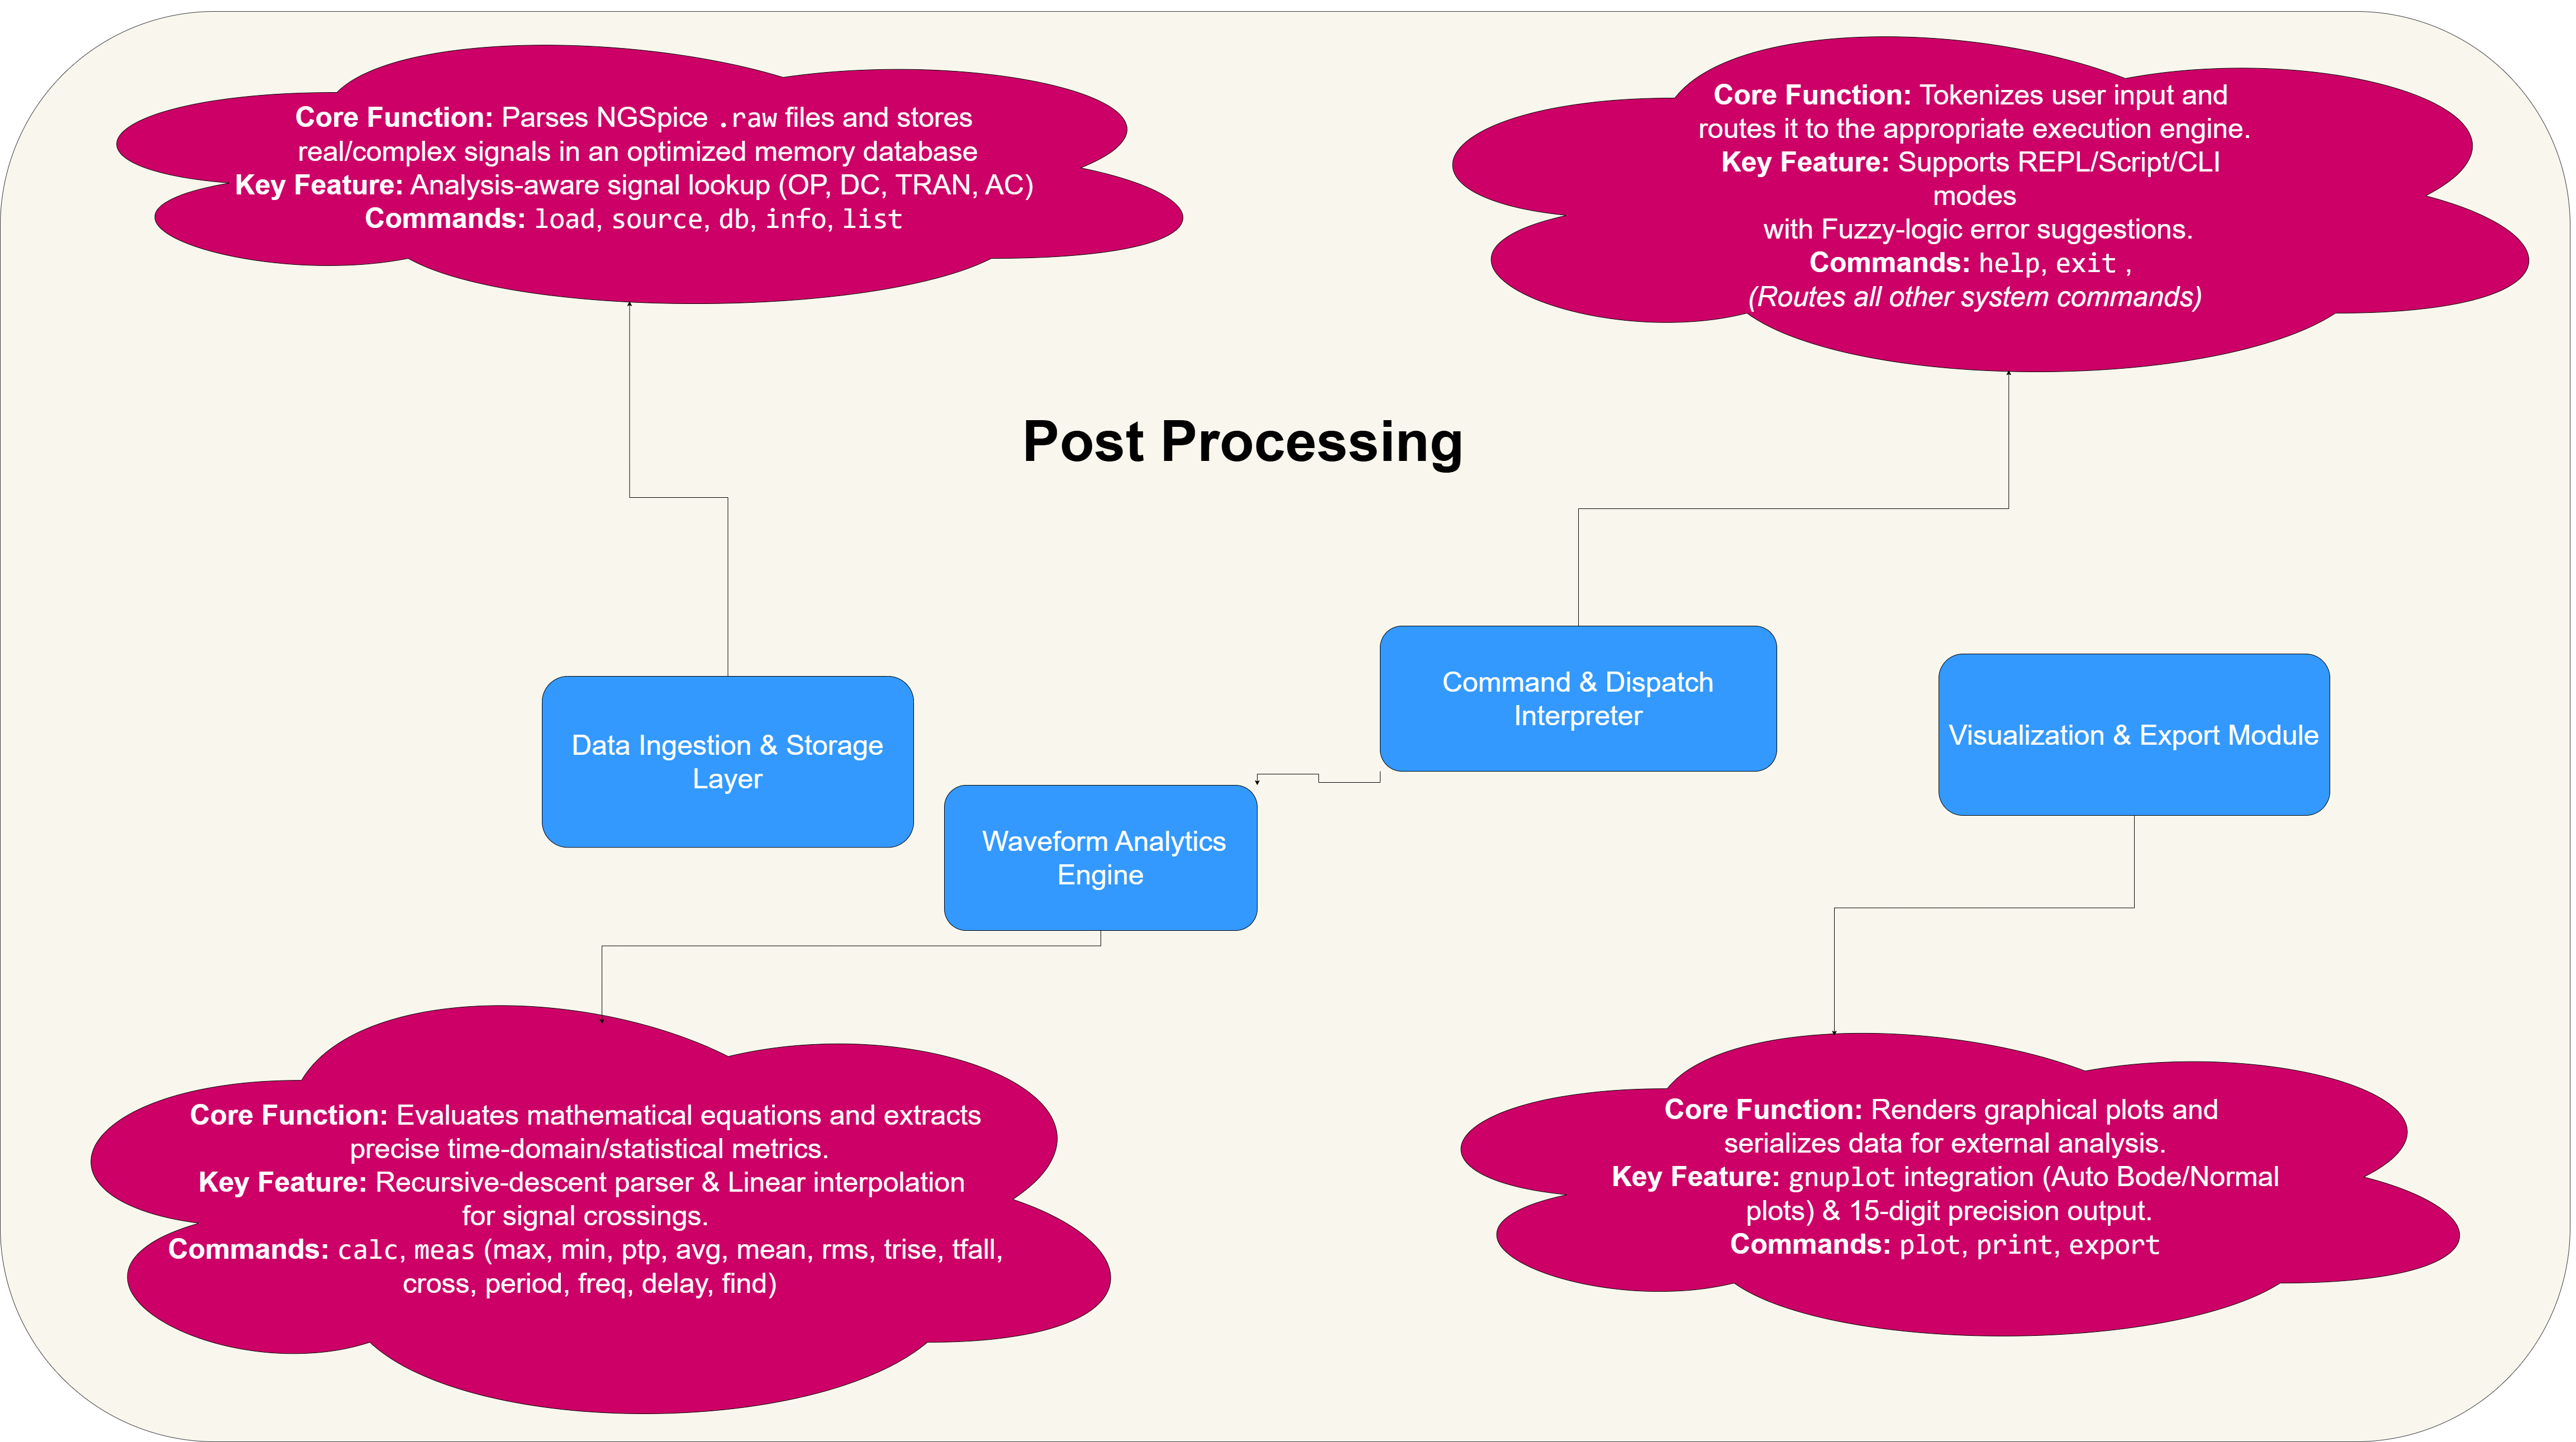
\includegraphics[width=0.8\textwidth]{Figures/Ch3/Postproc.drawio}
    \renewcommand{\thefigure}{3.3.4}
    \addtocounter{figure}{-1}
    \caption{ Post-Processing stage.}
    \label{fig:arch-postproc}
\end{figure}